%Estudio del comportamiento mecánico de una arteria

\subsection{Parte 1: Movimiento de una pared arterial}

Una arteria puede modelarse por un cilindro flexible de base circular, longitud $L$, radio $R_0$, cuyas paredes poseen un espesor $H$. Se supone que está constituido de un material elástico, incompresible, homogéneo e isotrópico. \\

Un modelo simplificado que describe el comportamiento mecánico de la pared arterial en interacción con el flujo sanguíneo se obtiene considerando que el cilindro es constituido por un conjunto de anillos independientes uno de otros. De esta manera se puede despreciar las interacciones longitudinales y axiales a lo largo de la arteria. Luego, se supone que la arteria se deforma solamente en la dirección radial. \\

El radio de la arteria está dado por,
\begin{equation}
R(t) = R_0 + y(t)
\end{equation}
donde $y(t)$ es la deformación radial en función del tiempo $t$. Al aplicar la ley de Newton en el sistema de anillo independientes conduce a una ecuación que permite modelar el comportamiento mecánico de la pared de la arteria en función del tiempo,
\begin{equation} \label{PROBLEMA_PARTE2}
\dfrac{d^2 y(t)}{dt^2} + \beta \dfrac{dy(t)}{dt} + \alpha y(t) = \gamma (p(t)-p_0)
\end{equation}
donde,
\begin{equation}
\alpha = \dfrac{E}{\rho_w R^2_0} \hspace{0,5cm} \gamma = \dfrac{1}{\rho_w H} \hspace{0,5cm} \beta = \mbox{constante} > 0 
\end{equation}

Particularmente se modela la variación de la presión a lo largo de la arteria como una función sinusoidal que depende de la posición $x$ y el instante de tiempo $t$,
\begin{equation} \label{FUENTE_PARTE2}
(p-p_0) = x \Delta p  \left( a + b cos( \omega_0 t ) \right)
\end{equation} 

\subsubsection*{Simulación 1}

Se calcula numericamente la ecuación (\ref{PROBLEMA_PARTE2}) con el término fuente (\ref{FUENTE_PARTE2}).  Se uyilizan los siguientes valores realistas para los parámetros físicos:
\begin{table} [H]
\centering
\begin{tabular}{llll}
$L$		& = $5 \times 10 ^ {-2}$ m 				&	$b$	 		&= $133.32$ N m $^{-2}$ \\
$R_0$	& = $5 \times 10 ^ {-3}$ m 				&	$a$		 	&= $1333.2$ N m $^{-2}$ \\
$\rho_w$& = $1 \times 10 ^ {3}$ kg m $^{-3}$ 	&	$\Delta p$ 	&= $33.33$ N m $^{-2}$ \\
$H$		& = $3 \times 10 ^ {-4}$ m 				&	$w_0$ 		&= $2 \pi / 0.8$ \\
$E$		& = $9 \times 10 ^ {5}$ N m $^{-2}$ 	&				&
\end{tabular}
\caption{Parametros utilizados para la simulación 1} \label{PARAMETROS_PARTE2}
\end{table}

Y considerando a su vez dos parametros de $\beta$:
\begin{enumerate}[label=(\alph*)]
\item $\beta = \sqrt{ \alpha }$ 
\item $\beta = \alpha$
\end{enumerate}

Se reescribe la ecuación (\ref{PROBLEMA_PARTE2}) como un sustema de ecuaciones lineales. En forma matricial,

\begin{equation} \label{PROBLEMA_PARTE2_CORREGIDO}
\vec{y'}(t) = \vect{A} \vec{y} + \vec{b}
\end{equation}

donde $\vec{y} = \begin{vmatrix} y & y' \end{vmatrix}^T$ ($T$ significa transpuesta), y $\vec{b}(t)$ es un vector fuente dependiente del tiempo $t$. La matriz $\vect{A}$ resultante es,

\begin{equation}
\vect{A} = \begin{pmatrix}
0 & 1 \\ -\alpha & -\beta
\end{pmatrix}
\end{equation}

Los valores propios de $\vect{A}$ se obtienen del desarrollo del polinomio característico,

\begin{equation}
det(\vect{A} - \lambda \vect{I}) = \begin{vmatrix}
-\lambda & 1 \\
-\alpha & -\lambda -\beta 
\end{vmatrix} \rightarrow \alpha \lambda^2 + \beta \lambda + 1 = 0
\end{equation}

Luego, los valores propios se calculan como la raíz del polinomio,

\begin{equation}
\lambda_{1,2} = \dfrac{( -\beta \pm \sqrt{ \beta^2 - 4 \alpha})}{2}
\end{equation}

Notar que para valores de $\beta \geq 2\sqrt{\alpha}$ ambos valores, $\lambda_1$ y $\lambda_2$, resultan reales y negativos, mientras que para valores de $\beta < 2\sqrt{\alpha}$ ambos autovalores resultan números complejos con su componente real negativa. \\

Se implementa una subrutina que permite calcular los valores propios de la matriz $\vect{A}$. Utilizando los valores de la Tabla \ref{PARAMETROS_PARTE2} se obtiene:
\begin{enumerate} [label=(\alph*)]
\item $\beta = \sqrt{\alpha} = 6.0 \times 10^3 $
\begin{equation}
\vect{A} = \begin{pmatrix} 0 & 1 \\ 36.0 \times 10^6 & 6.0 \times 10^3 \end{pmatrix} \rightarrow 
\begin{matrix} \lambda_1 = & -3000.00 + 5196.15 i \\ \lambda_2 = & -3000.00 - 5196.15 i \end{matrix}
\end{equation} 
\item $\beta = \alpha =  36.0 \times 10^6 $
\begin{equation}
\vect{A} = \begin{pmatrix} 0 & 1 \\ 36.0 \times 10^6 & 36.0 \times 10^6 \end{pmatrix} \rightarrow 
\begin{matrix} \lambda_1 = & -1.0 \\ \lambda_2 = & -36.0 \times 10^6 \end{matrix}
\end{equation} 
\end{enumerate}

%------------------------------------

\subsubsection{Simulación 1: Euler Implicito} 

\paragraph{Discretización de la ecuación diferencial}
Se implementa una subrutina que permite calcular la ecuacion (\ref{PROBLEMA_PARTE2}) usando el método de Euler Implícito para dos valores de $\beta$. Sea $y(x,t) = y^n_j$ y $\partial y / \partial t (x,t) = z^n_j$, recurriendo a la expresión (\ref{PROBLEMA_PARTE2_CORREGIDO}) e implementando un esquema de integración implícito se tiene que,
\begin{align}
\dfrac{y^n - y^{n-1}}{\Delta t} &= z^n \\
\dfrac{z^n - z^{n-1}}{\Delta t} &= -\alpha y^n - \beta z^n + \gamma (p_n-p_0)
\end{align}

Reordenando los valores en los pasos de tiempo $n$ y $n-1$ en los lados izquierdo y derecho respectivamente, se expresa la relación anterior en forma matricial como,
\begin{equation}
\vect{A} \cdot \begin{Bmatrix}
y^n \\ z^n
\end{Bmatrix} =
\begin{Bmatrix}
y^{n-1} \\ z^{n-1}
\end{Bmatrix} +
\Delta t \begin{Bmatrix}
0 \\ \gamma (p_n-p_0)
\end{Bmatrix}
\end{equation}
donde,
\begin{equation}
\vect{A} = \begin{pmatrix}
1 & -\Delta t \\
\Delta t \alpha & 1+ \Delta t \beta
\end{pmatrix}
\end{equation}

Despenjando las incognitas $\begin{Bmatrix} y^n & z^n \end{Bmatrix} ^T$ se obtiene,
\begin{equation}
\begin{Bmatrix}
y^n \\ z^n
\end{Bmatrix} =
\vect{A}^{-1} \cdot \begin{Bmatrix}
y^{n-1} \\ z^{n-1}
\end{Bmatrix} +
\Delta t \vect{A}^{-1} \cdot  \begin{Bmatrix}
0 \\ \gamma (p_n-p_0)
\end{Bmatrix}
\end{equation}
donde
\begin{equation}
\vect{A}^{-1} = 
\dfrac{1}{1 + \beta \Delta t + \alpha (\Delta t) ^ 2}
\begin{pmatrix}
1+\beta \Delta t & \Delta t \\
-\Delta t \alpha & 1 
\end{pmatrix}
\end{equation}

\paragraph{Estabilidad de la solución}
Se quiere estudiar la estabilidad de la solución transiente de (\ref{PROBLEMA_PARTE2_CORREGIDO}). Para ello se recurre a las expresiones (\ref{analisis_espectral_general}) y (\ref{analisis_espectral_descompuesto}). Luego,
\begin{align}
\dfrac{ y^{n+1} - y^n } { \Delta t } & = \Omega_1 y^{n+1} \\
\dfrac{ z^{n+1} - z^n } { \Delta t } & = \Omega_2 z^{n+1}
\end{align} 

\begin{equation}
\dfrac{d \vec{U}}{d t} = \vect{S} \vec{U} + \vec{Q} \rightarrow \left\{ \begin{matrix}
( y^{n+1} - y^n ) /  \Delta t  = \Omega_1 y^{n+1} \\
( z^{n+1} - z^n ) /  \Delta t  = \Omega_2 z^{n+1}
\end{matrix} \right.
\end{equation}

Despejando los terminos evaluados en $t_{n+1}$ en la izquierda de la ecuación

\begin{align}
y^{n+1} &= \dfrac{ 1 }{ 1 - \Delta t \Omega_1 } y^n \\
z^{n+1} &= \dfrac{ 1 }{ 1 - \Delta t \Omega_2 } z^n
\end{align}

Se reconocen los términos $\vec{z}_p$ para $y$ y $z$. Teniendo en cuenta los valores propios $\Omega$ antes calculado

\begin{align}
z_p &= \dfrac{1}{1-\Omega_j \Delta t} \\
&= \dfrac{1}{ \left[ 1-\Re(\Omega_j) \Delta t \right] - \left[ \Im(\Omega_j) \Delta t \right] i }\\
&= \dfrac{\left[ 1- \Re(\Omega_j) \Delta t \right] + \left[ \Im(\Omega_j) \Delta t \right] i }{ \left[ 1-\Re(\Omega_j) \Delta t \right]^2 + \left[ \Im(\Omega_j) \Delta t \right]^2}
\end{align}

El módulo de $z_p$ viene dado por

\begin{equation}
||z_p|| = \dfrac{ \sqrt{ \left[ 1-\Re(\Omega_j) \Delta t \right]^2 + \left[ \Im(\Omega_j) \Delta t \right]^2 } } { \left[ 1- \Re(\Omega_j) \Delta t \right]^2 + \left[ \Im(\Omega_j) \Delta t \right]^2}
\end{equation}

\begin{enumerate}[label=(\alph*)]

\item $\beta = \alpha$ y $\Delta t = 10^4$
\begin{center}
\begin{tabular}{lll}
$\Omega_1 = −3000.00 + 5196.15i$ & $\rightarrow$ & $z_{p1} = $ \\
$\Omega_2 = −3000.00 - 5196.15i$ & $\rightarrow$ & $z_{p2} = $
\end{tabular}
\end{center}

\item $\beta = \sqrt{\alpha}$ y $\Delta t = 10^4$
\begin{center}
\begin{tabular}{lll}
$\Omega_1 = -1.0$ & $\rightarrow$ & $z_{p1} = $ \\
$\Omega_2 = -36.0 \times 10^6$ & $\rightarrow$ & $z_{p2} = $
\end{tabular}
\end{center}

\end{enumerate}



%----------------------- FIGURAS SIMULACION 1 -----------------------------
%----------------------- 	EULER IMPLICITO  -----------------------------

\begin{center}
\begin{figure} [H]
	\begin{subfigure}[b]{0.3\textwidth}
		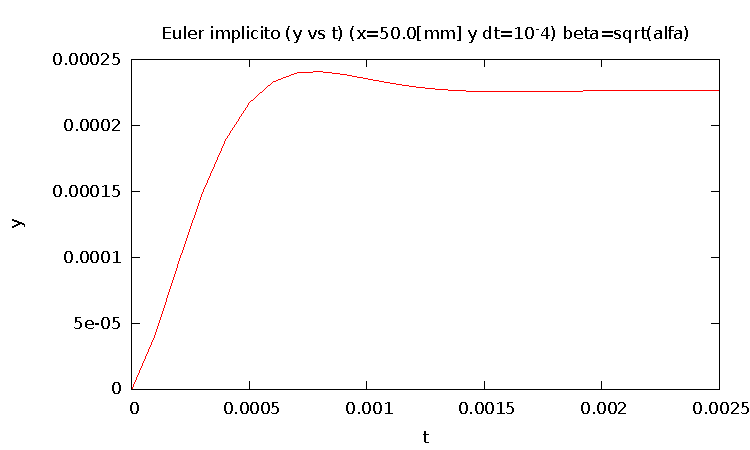
\includegraphics{./parte3/graficos/grafico_euler_S1_y_b1.pdf}
		\caption{} 
		\label{fig:eulerS1b1_y}
	\end{subfigure}
	
	\begin{subfigure}[b]{0.3\textwidth}
		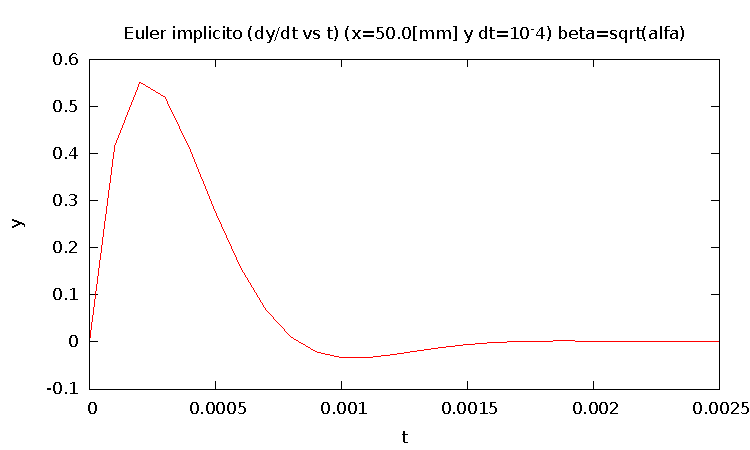
\includegraphics{./parte3/graficos/grafico_euler_S1_dy_b1.pdf}
		\caption{} 
		\label{fig:eulerS1b1_dy}
	\end{subfigure}
\caption{} \label{euler_S1_b1}
\end{figure}
\end{center}


\begin{center}
\begin{figure} [H]
	\begin{subfigure}[b]{0.3\textwidth}
		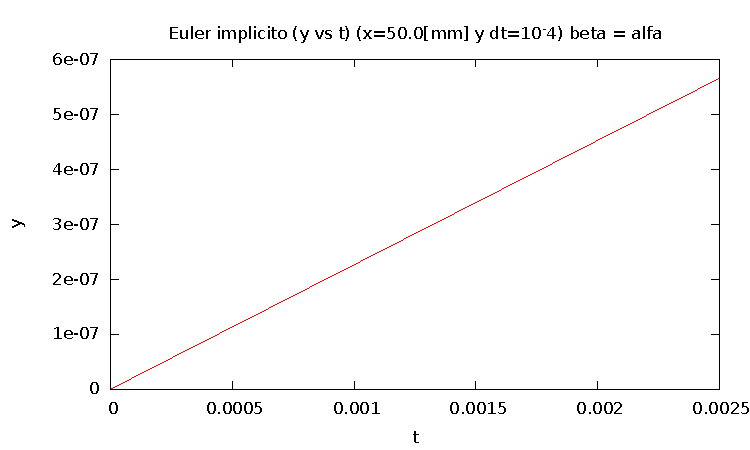
\includegraphics{./parte3/graficos/grafico_euler_S1_y_b2.pdf}
		\caption{} 
		\label{fig:eulerS1b2_y}
	\end{subfigure}
	
	\begin{subfigure}[b]{0.3\textwidth}
		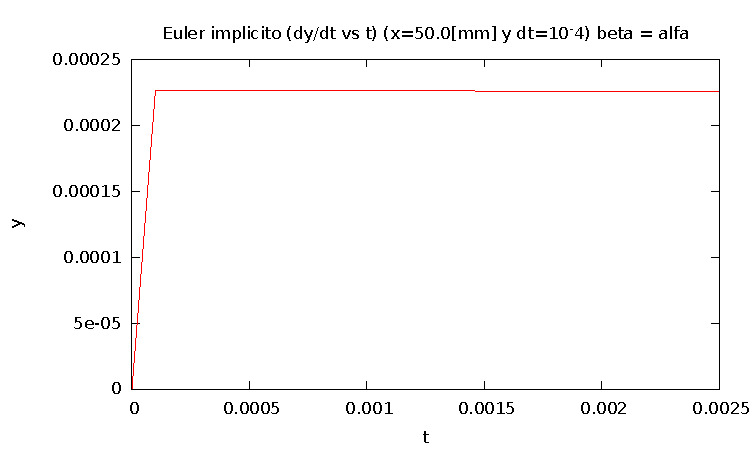
\includegraphics{./parte3/graficos/grafico_euler_S1_dy_b2.pdf}
		\caption{} 
		\label{fig:eulerS1b2_dy}
	\end{subfigure}
\caption{} \label{euler_S1_b2}
\end{figure}
\end{center}

%----------------------------------------------------------------------------

\subsubsection{Simulación 1: Crank Nicolson}

Discretizacion de la ecuación por el método Crank Nicolson

\begin{align}
\dfrac{y^{n+1}-y^n}{\Delta t} & = \dfrac{1}{2} \left( z^{n+1} + z^n \right) \\
\dfrac{z^{n+1}-z^n}{\Delta t} &= \dfrac{1}{2} \left( -\alpha y^{n+1} - \beta y^{n+1} + \gamma (p_{n+1}-p_0) \right) + \dfrac{1}{2} \left( -\alpha y^{n} - \beta y^{n} + \gamma (p_{n}-p_0) \right)  
\end{align}

La relación anterior se escribe en forma matricial,

\begin{equation}
\vect{A} \cdot
\begin{Bmatrix}
y^{n+1} \\ z^{n+1}
\end{Bmatrix} =
\vect{B} \cdot
\begin{Bmatrix}
y^n \\ z^n
\end{Bmatrix} + \dfrac{\Delta t}{2}
\begin{Bmatrix}
0 \\ \left( \gamma (p_{n+1}-p_0) + \gamma (p_{n}-p_0) \right)
\end{Bmatrix}
\end{equation}

donde,

\begin{equation}
\vect{A} = \begin{pmatrix}
1 & -\dfrac{\Delta t}{2} \\
\dfrac{\alpha \Delta t}{2} & 1+ \dfrac{\beta \Delta t}{2}
\end{pmatrix} 
\end{equation}

\begin{equation}
\vect{B} = \begin{pmatrix}
1 & \dfrac{\Delta t}{2} \\
-\dfrac{\alpha \Delta t}{2} & 1-\dfrac{\beta \Delta t}{2}
\end{pmatrix}
\end{equation}

Despejando las variables incognitas se obtiene,

\begin{equation}
\begin{Bmatrix}
y^{n+1} \\ z^{n+1} 
\end{Bmatrix} =
\vect{A}^{n-1} \cdot \vect{B} \cdot 
\begin{Bmatrix}
y^n \\ z^n 
\end{Bmatrix} + \dfrac{\Delta t}{2} \vect{A}^{-1} \cdot
\begin{Bmatrix}
0 \\ \left( \gamma (p_{n+1}-p_0) + \gamma (p_{n}-p_0) \right)
\end{Bmatrix}
\end{equation}

donde 

\begin{equation}
\vect{A}^{-1} = \dfrac{1}{1 + \beta \dfrac{\Delta t}{2} + \alpha \left( \dfrac{\Delta t}{2} \right)^2 } 
\begin{pmatrix}
1 + \dfrac{\beta \Delta t}{2} & \dfrac{\Delta t}{2}\\
-\dfrac{\alpha \Delta t}{2} & 1 
\end{pmatrix}
\end{equation}

Se grafican los resultados y se exponen en las Figura \ref{cn_S1_b1} y \ref{cn_S1_b2}

Se quiere estudiar la estabilidad de la solución transiente (homogénea) de (QUE ECUACIÓN). Para ello se ...

\begin{align}
\dfrac{ y^{n+1} - y^n } { \Delta t } & = \Omega_1 \dfrac{1}{2} \left( y^{n+1} + y^{n} \right) \\
\dfrac{ z^{n+1} - z^n } { \Delta t } & = \Omega_2 \dfrac{1}{2} \left( z^{n+1} + z^{n} \right)
\end{align} 

Despejando los terminos evaluados en $t_{n+1}$ en la izquierda de la ecuación

\begin{align}
y^{n+1} &= \dfrac{ 1 + \Delta t \Omega_1 }{ 1 - \Delta t \Omega_1 } y^n \\
z^{n+1} &= \dfrac{ 1 + \Delta t \Omega_2 }{ 1 - \Delta t \Omega_2 } z^n
\end{align}

Se reconocen los términos $\vec{z}_p$ para $y$ y $z$. Teniendo en cuenta los valores propios $\Omega$ antes calculado

\begin{align}
z_p &= \dfrac{1+\Omega_j \Delta t}{1-\Omega_j \Delta t / 2} \\
&= \dfrac{\left[ 1-\Re(\Omega_j) \Delta t / 2 \right] + \left[ \Im(\Omega_j) \Delta t / 2 \right] i}
		 {\left[ 1- \Re(\Omega_j) \Delta t / 2 \right] - \left[ \Im(\Omega_j) \Delta t / 2 \right] i} \\
&= \dfrac{\left[ \left( 1- \Re(\Omega_j) \Delta t / 2 \right) + \left( \Im(\Omega_j) \Delta t / 2 \right) i \right] \cdot \left[ \left( 1+ \Re(\Omega_j) \Delta t / 2 \right) + \left( \Im(\Omega_j) \Delta t / 2 \right) i \right]}
		 {\left[ 1- \Re(\Omega_j) \Delta t / 2 \right]^2 + \left[ \Im(\Omega_j) \Delta t / 2 \right]^2} \\
&= \dfrac{ \left[ 1 - \Re(\Omega_j)\Delta t / 2 - \Im(\Omega_j)\Delta t / 2 \right] + \left[ \Im (\Omega_j) \Delta t / 2 \right] i  } {\left[ 1-\Delta t \Re(\Omega_j) \right]^2 + \left[ \Delta t \Im(\Omega_j) \right]^2}
\end{align}

El módulo de $z_p$ viene dado por

\begin{equation}
||z_p|| = \dfrac{ \sqrt{ \left[ 1 - \dfrac{\Re(\Omega_j)\Delta t}{2} - \dfrac{\Im(\Omega_j)\Delta t}{2} \right]^2 + \left[ \dfrac{\Im \Delta t}{2}\right]^2 } } {\left[ \dfrac{1-\Delta t \Re(\Omega_j)}{2} \right]^2 + \left[ \dfrac{\Delta t \Im(\Omega_j)}{2} \right]^2}
\end{equation}

\begin{enumerate}[label=(\alph*)]

\item $\beta = \alpha$ y $\Delta t = 10^4$
\begin{center}
\begin{tabular}{lll}
$\Omega_1 = −3000.00 + 5196.15i$ & $\rightarrow$ & $z_{p1} = $ \\
$\Omega_2 = −3000.00 - 5196.15i$ & $\rightarrow$ & $z_{p2} = $
\end{tabular}
\end{center}

\item $\beta = \sqrt{\alpha}$ y $\Delta t = 10^4$
\begin{center}
\begin{tabular}{lll}
$\Omega_1 = -1.0$ & $\rightarrow$ & $z_{p1} = $ \\
$\Omega_2 = -36.0 \times 10^6$ & $\rightarrow$ & $z_{p2} = $
\end{tabular}
\end{center}

\end{enumerate}

%----------------------- FIGURAS SIMULACION 1 -----------------------------
%----------------------- 	CRANK NICOLSON -----------------------------

\begin{center}
\begin{figure} [H]
	\begin{subfigure}[b]{0.3\textwidth}
		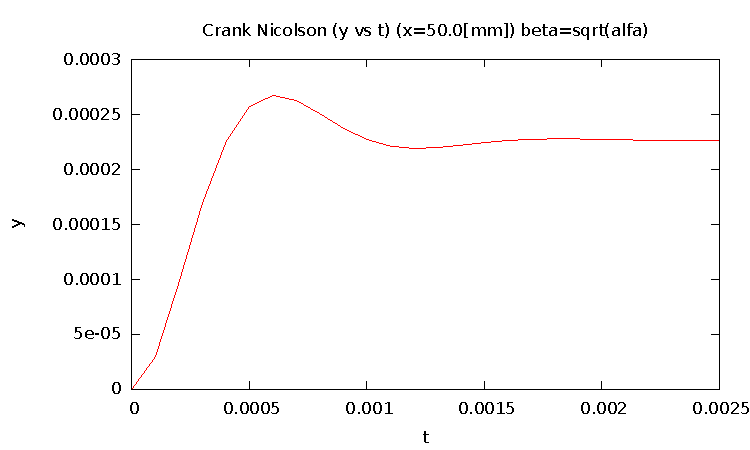
\includegraphics{./parte3/graficos/grafico_cn_S1_y_b1.pdf}
		\caption{} 
		\label{fig:cnS1b1_y}
	\end{subfigure}
	
	\begin{subfigure}[b]{0.3\textwidth}
		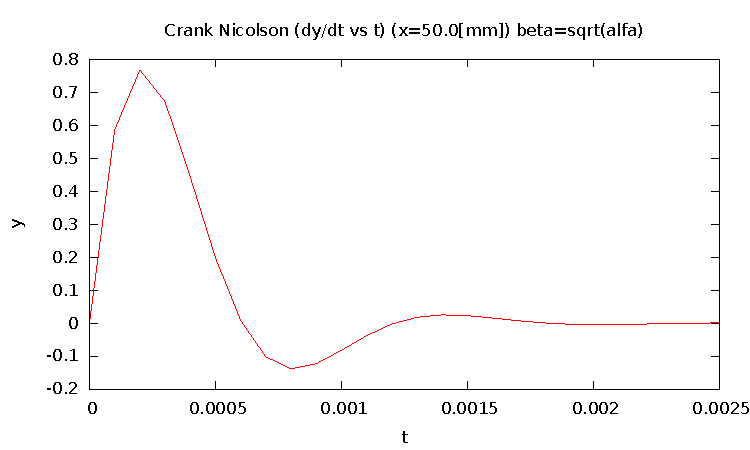
\includegraphics{./parte3/graficos/grafico_cn_S1_dy_b1.pdf}
		\caption{} 
		\label{fig:cnS1b1_dy}
	\end{subfigure}
\caption{} \label{cn_S1_b1}
\end{figure}
\end{center}

\begin{center}
\begin{figure} [H]
	\begin{subfigure}[b]{0.3\textwidth}
		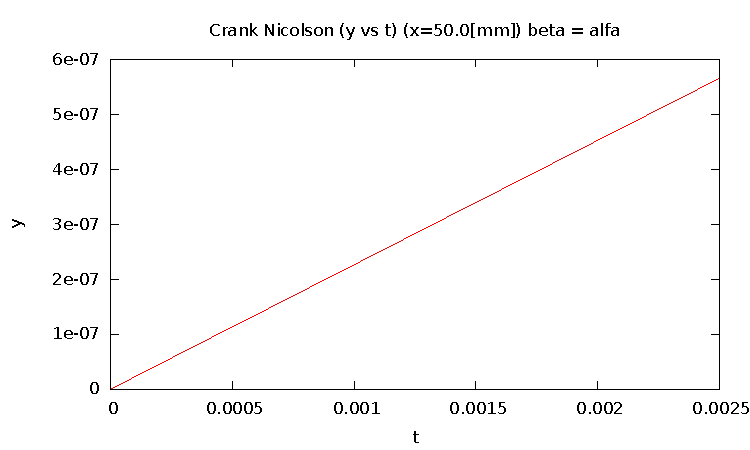
\includegraphics{./parte3/graficos/grafico_cn_S1_y_b2.pdf}
		\caption{} 
		\label{fig:cnS1b2_y}
	\end{subfigure}
	
	\begin{subfigure}[b]{0.3\textwidth}
		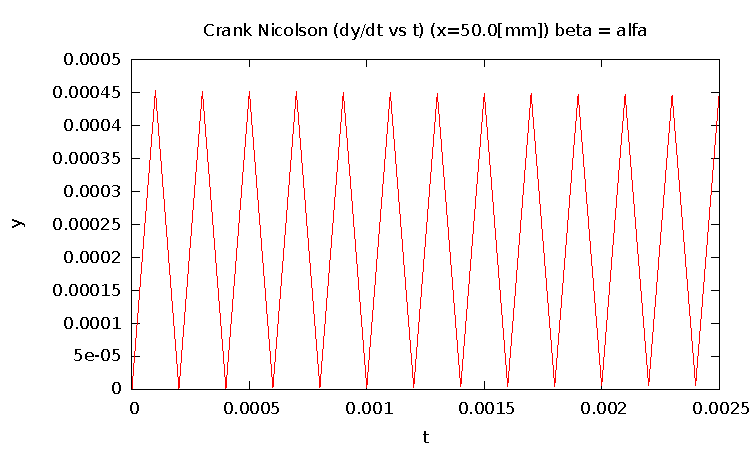
\includegraphics{./parte3/graficos/grafico_cn_S1_dy_b2.pdf}
		\caption{} 
		\label{fig:cnS1b2_dy}
	\end{subfigure}
\caption{} \label{cn_S1_b2}
\end{figure}
\end{center}

%-------------------------------------------------------------------------

\subsubsection{Simulación 2}

%----------------------- FIGURAS SIMULACION 2 -----------------------------
%----------------------- 	EULER IMPLICITO  -----------------------------

\begin{center}
\begin{figure} [H]
	\begin{subfigure}[b]{0.3\textwidth}
		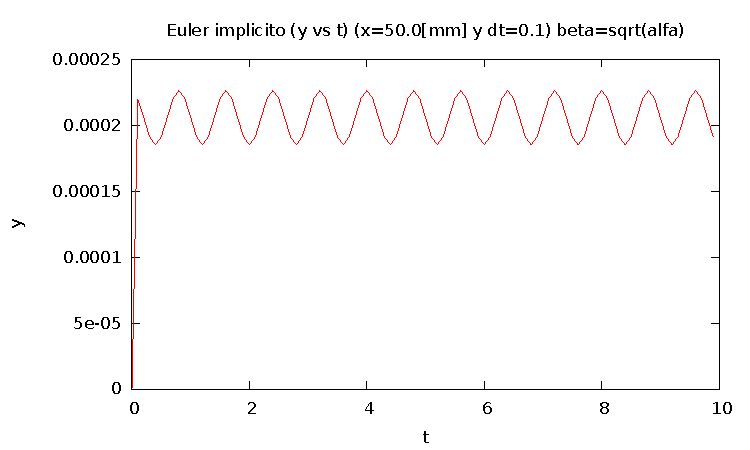
\includegraphics{./parte3/graficos/grafico_euler_S2_y_b1.pdf}
		\caption{} 
		\label{fig:eulerS2b1_y}
	\end{subfigure}
	
	\begin{subfigure}[b]{0.3\textwidth}
		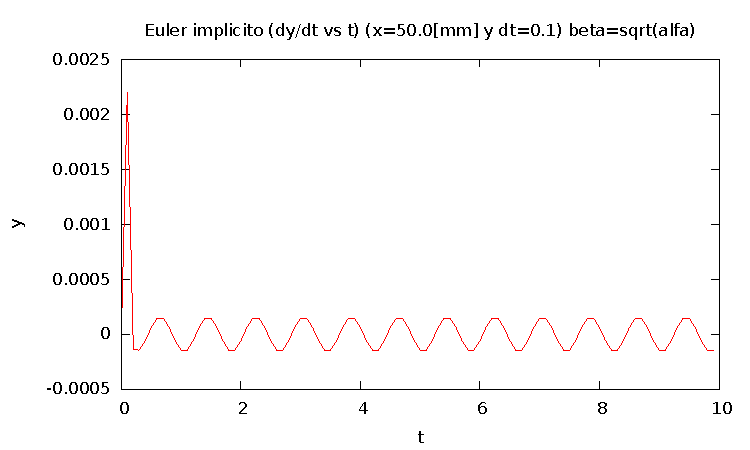
\includegraphics{./parte3/graficos/grafico_euler_S2_dy_b1.pdf}
		\caption{} 
		\label{fig:eulerS2b1_dy}
	\end{subfigure}
\end{figure}
\end{center}

\begin{center}
\begin{figure} [H]
	\begin{subfigure}[b]{0.3\textwidth}
		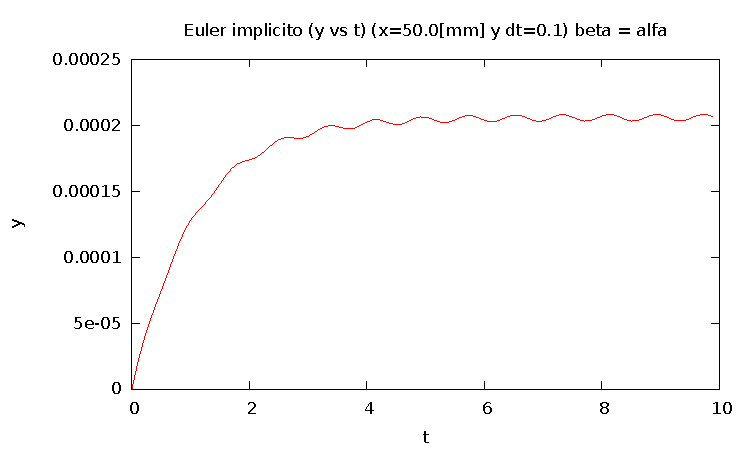
\includegraphics{./parte3/graficos/grafico_euler_S2_y_b2.pdf}
		\caption{} 
		\label{fig:eulerS2b2_y}
	\end{subfigure}
	
	\begin{subfigure}[b]{0.3\textwidth}
		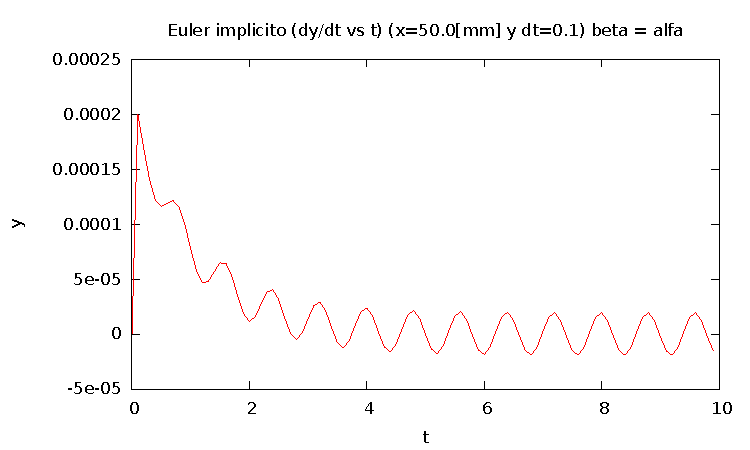
\includegraphics{./parte3/graficos/grafico_euler_S2_dy_b2.pdf}
		\caption{} 
		\label{fig:eulerS2b2_dy}
	\end{subfigure}
\end{figure}
\end{center}

%--------------------------------------------------------------------------


%----------------------- FIGURAS SIMULACION 2 -----------------------------
%-----------------------	CRANK NICOLSON -----------------------------

\begin{center}
\begin{figure} [H]
	\begin{subfigure}[b]{0.3\textwidth}
		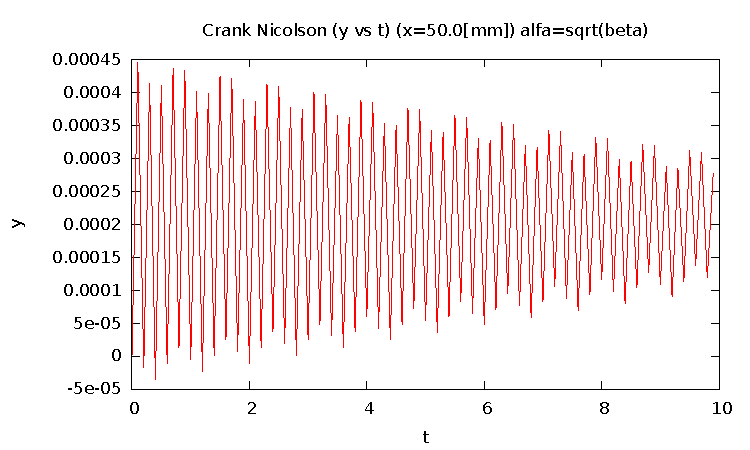
\includegraphics{./parte3/graficos/grafico_cn_S2_y_b1.pdf}
		\caption{} 
		\label{fig:cnS2b1_y}
	\end{subfigure}
	
	\begin{subfigure}[b]{0.3\textwidth}
		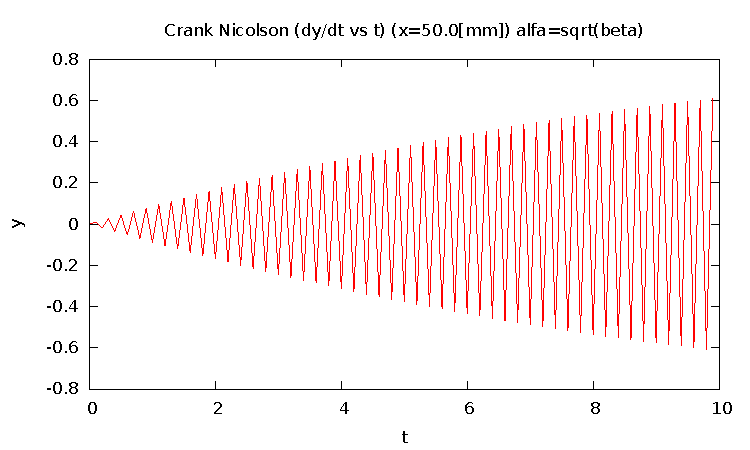
\includegraphics{./parte3/graficos/grafico_cn_S2_dy_b1.pdf}
		\caption{} 
		\label{fig:cnS2b1_dy}
	\end{subfigure}
\end{figure}
\end{center}

\begin{center}
\begin{figure} [H]
	\begin{subfigure}[b]{0.3\textwidth}
		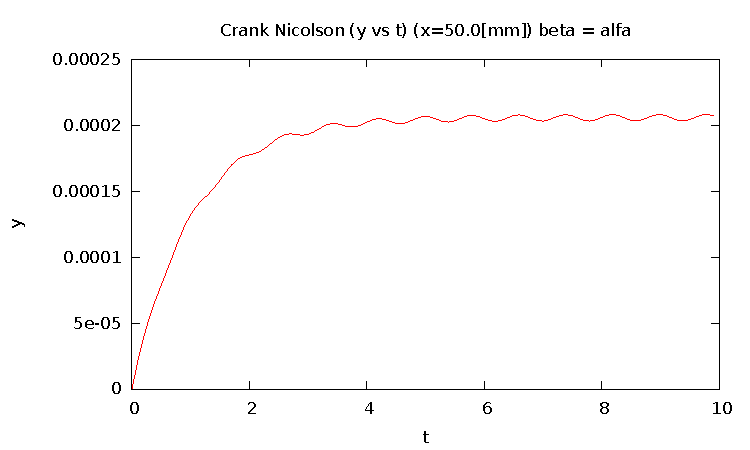
\includegraphics{./parte3/graficos/grafico_cn_S2_y_b2.pdf}
		\caption{} 
		\label{fig:cnS2b2_y}
	\end{subfigure}
	
	\begin{subfigure}[b]{0.3\textwidth}
		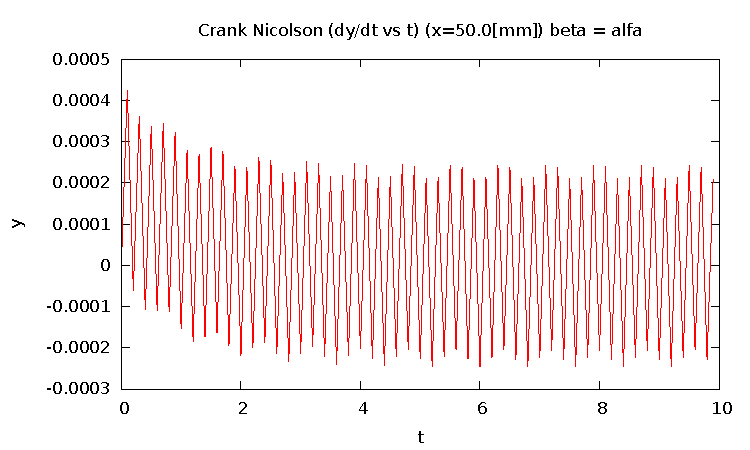
\includegraphics{./parte3/graficos/grafico_cn_S2_dy_b2.pdf}
		\caption{} 
		\label{fig:cnS2b2_dy}
	\end{subfigure}
\end{figure}

\end{center}

%------------------------------------------------------------------------

COMENTAR RESULTADOS Y ESTUDIAR SI ES POSIBLE UTILIZAR UNA SOLUCIÓN 